\chapter{Eksperimen dan Evaluasi}

Bab ini menjelaskan tahapan implementasi pembangunan model, konfigurasi eksperimen, dan evaluasi kinerja model berdasarkan hasil eksperimen yang dilakukan.


\section{Tujuan Eksperimen}

Eksperimen dalam penelitian ini dilakukan dalam penentuan model bahasa dan parameter model, dan juga untuk mengukur kinerja model ASR, VSR, dan AVSR yang dibangun. Kinerja yang diukur adalah hasil pembangkitan kalimat yang ditranskripsikan dari suara dan gambar pada video. Kinerja tersebut diukur dengan menggunakan metrik \textit{word error rate} (WER). Kualitas pembangkitan transkripsi dinilai baik jika memilki WER yang rendah.


\section{Pembangunan Model}
\label{sec:pembangunan-model}

Berdasarkan hasil eksperimen yang dilakukan, dibangun model ASR, VSR, dan AVSR yang sesuai untuk mengenali ucapan dalam bahasa Indonesia.


\subsection{Persiapan dan Pembentukan Transkripsi}

\begin{figure}[h]
    \centering
    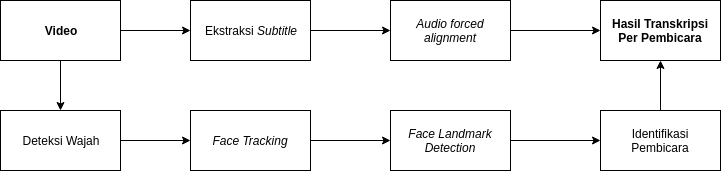
\includegraphics[width=0.8\textwidth]{resources/images/proses-persiapan-transkripsi.png}
    \caption{Alur proses persiapan transkripsi.}
    \label{fig:proses-persiapan-transkripsi}
\end{figure}

Untuk melatih model diperlukan transkripsi dengan cap waktu yang selaras dengan suara yang diucapkan. Beberapa video di YouTube sudah ada yang menyediakan \textit{subtitle} dan juga sudah selaras waktunya dengan kata-kata yang diucapkan di video. Akan tetapi subtitle tersebut hanya memiliki cap waktu dalam satuan kalimat, tidak kata per kata, sehingga perlu dilakukan penyelarasan menggunakan Penn Phonetics Lab Forced Aligner (dibangun berdasarkan kakas sumber terbuka HTK \textit{Toolbox}). Teks yang akan diselaraskan merupakan teks dari \textit{subtitle} yang kemudian dipetakan menjadi cara pelafalannya dengan kamus pelafalan yang sudah dibuat dengan menggunakan kakas Corpus Management Tools. Kakas penyelaras tersebut menggunakan algoritma Viterbi untuk menghitung \textit{maximum likelihood alignment} antara audio (yang dimodelkan menggunakan fitur PLP) dengan teks.


\subsection{Persiapan Korpus Video}

\begin{figure}[h]
    \centering
    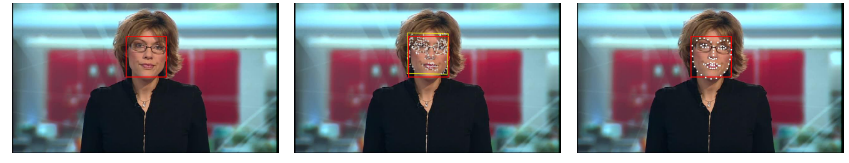
\includegraphics[width=0.8\textwidth]{resources/images/face-detection.png}
    \caption{\textbf{Kiri:} Pendeteksian wajah (\textit{bounding box} merah). \textbf{Tengah:} \textit{tracking} wajah menggunakan fitur KLT (\textit{bounding box} kuning). \textbf{Kanan:} Pendeteksian \textit{landmark} wajah.}
    \label{fig:face-detection}
\end{figure}

Corpus video yang telah dikumpulkan dideteksi wajah-wajah yang terdapat pada setiap framenya menggunakan metode berbasis HOG. Setelah wajah berhasil dideteksi, masing-masing wajah tersebut di\textit{tracking} menggunakan KLT \textit{tracker}, yang berguna juga dalam mengurangi \textit{false positive} pada saat tahap pendeteksian wajah. Kemudian dari wajah yang sudah terdeteksi tersebut dideteksi \textit{landmark}nya, yang kemudian \textit{landmark} tersebut bisa digunakan untuk menentukan posisi mulut pada wajah. Untuk menentukan siapa yang sedang berbicara pada video, ditentukan dengan cara menghitung jarak ternormalisasi antara bibir atas dan bibir bawah dari setiap wajah yang terdeteksi, dan juga dihitung frekuensi buka tutup dari bibirnya.


\subsection{Ekstraksi Fitur}

Terdapat dua ekstraksi fitur yang digunakan dalam penelitian ini, yaitu MFCC yang digunakan untuk mengektrasi fitur audio, dan CNN yang digunakan untuk mengektraksi fitur frame pada video. Konfigurasi parameter dari MFCC menggunakan  36-MFCC berdasarkan penelitian \textcite{Yuwan2018} dan untuk konfigurasi parameter CNN menggunakan konfigurasi pada penelitian \textcite{Chung2017}.


\subsection{Eksperimen Pemodelan Sekuens}

Pada eksperimen pemodelan sekuens, sekuens akan memodelkan dari tiga jenis masukan, yaitu masukan akustik saja, masukan visual saja, dan masukan gabungan akustik dan visual. Akan tetapi arsitektur model dari sekuensnya itu sendiri tetap sama, sehingga parameter-parameter yang bisa diuji pun jumlahnya akan tetap sama. Pemodelan sekuens yang digunakan adalah model transformer dan diimplementasikan dengan menggunakan TensorFlow dan PyTorch, yang disediakan oleh \textcite{Dai2019} pada laman GitHub \footnote{\url{https://github.com/kimiyoung/transformer-xl}}.
\bigskip

Sebelum pemodelan sekuens dilakukan, perlu dilakukan proses ekstraksi fitur seperti yang sudah dijelaskan sebelumnya. Setelah itu, model transformer dibentuk dengan menggunakan perintah

\begin{verbatim}
    bash run_enwik8_base.sh train --work_dir PATH_TO_WORK_DIR
\end{verbatim}

untuk melakukan proses pelatihan dan menggunakan perintah

\begin{verbatim}
    bash run_enwik8_base.sh eval --work_dir PATH_TO_WORK_DIR
\end{verbatim}

untuk melakukan proses evaluasi. \verb|PATH_TO_WORK_DIR| adalah direktori tempat hasil pemodelan disimpan. Selain itu ada juga opsi-opsi tambahan yang diuji seperti 
\begin{itemize}
    \item \verb|--batch_chuck| untuk menukar performa kecepatan pelatihan dengan memori yang digunakan. Untuk \verb|batch_chuck>1|, program akan membagi setiap data latih menjadi \verb|batch_chuck| bagian dan melakukan pelatihan pada setiap \textit{batch} secara berurutan, dan gradien yang terkumpul akan dibagi dengan jumlah \verb|batch_chuck|.
    \item \verb|--div_val| untuk mengurangi dimensi \textit{embedding}.
    \item \verb|--fp16| dan \verb|--dynamic-loss-scale| untuk menjalankan pelatihan dengan menggunakan mode pseudo-fp16 dan \textit{dynamic loss scaling}. Untuk penggunaan \verb|--fp16| perlu dilakukan pemasangan \textit{package} \verb|apex|\footnote{\url{https://github.com/NVIDIA/apex/}} terlebih dahulu.
    \item \verb|mem_len=0| untuk melakukan pelatihan tanpa menggunakan mekanisme rekurens.
    \item \verb|attn_type=2| untuk melakukan pelatihan dengan model transformer standar tanpa menggunakan \textit{positional encoding} relatif.
\end{itemize}

\section{Skenario Eksperimen}

Proses pengujian dibagi menjadi tiga tahap. Pengujian pertama dilakukan terhadap pembangkitan transkripsi menggunakan model akustik. Pengujian kedua dilakukan terhadap pembangkitan transkripsi menggunakan model visual. Terakhir, pengujian ketiga dilakukan terhadap pembangkitan transkripsi menggunakan model akustik dan model visual.

\section{Hasil Eksperimen dan Evaluasi}

Upabab ini membahas tentang hasil eksperimen pemodelan sekuens sesuai dengan implementasi pada upabab \ref{sec:pembangunan-model}

\subsection{Parameter Model ASR}

\subsection{Parameter Model VSR}

\subsection{Parameter Model AVSR}